\documentclass[runningheads]{llncs}
\usepackage{graphicx}
\usepackage{lipsum}
\usepackage{amsmath}

\begin{document}

\chapter{[Chapter 4] Evaluation}

Success criteria from the project proposal:

\begin{itemize}

\item Implement all basic modules: Object modelling, Collision detection, Bounce, Friction, Stability.

\item Evaluate the engine by comparing it with popular existing engines with simple experiments.

\item Demonstrate that the engine works with screenshots of simple examples.
\end{itemize}

For extensions (ordered by priority):

\begin{itemize}
\item Implement fluid dynamics.

\item Implement different versions of the engine for whether GPU is used, and for other interesting parameters like the number of cores used. 
Then evaluate the performance.

\item Implement real-time rendering, which should allow the project to meet all previous criteria without third-party rendering libraries. 

\item Implement soft-body dynamics.


Evaluation of physics engines in general can be quite challenging, 
especially for quantitative analysis.
Little work has been done in this area as of now, 
likely due to the complexity, systematic bias, and the lack of needs.

The evaluation of this project is split into three parts: Benchmark selection, Quantitative analysis, and Qualitative analysis.

\section{Benchmark selection}

Quantitative evaluations will be largely comparison-based. 
I will be choosing at least three open-source physics engines that support similar features to compare against.
The following engines have been found as possible candidates:

\begin{table}[h]
  \centering
  \makebox[\linewidth]{
  \begin{tabular}
  {|c|c|}
  \hline 
  Physics engine                                & Website                                                         \\
  \hline 
  Advanced Simulation Library                   & asl.org.il                                           \\
  Bullet                                        & pybullet.org                                           \\
  Newton Game Dynamics                          & newtondynamics.com/forum/newton.php                      \\
  Open Dynamics Engine                          & www.ode.org                                            \\
  PAL              & www.adrianboeing.com/pal                                \\
  PhysX                                         & www.nvidia.com/en-gb/geforce/technologies/physx        \\
  Project Chrono~                               & projectchrono.org                                      \\
  Siconos                                       & nonsmooth.gricad-pages.univ-grenoble-alpes.fr/siconos  \\
  SOFA & www.sofa-framework.org                                 \\
  Tokamak physics engine                        & github.com/isegal/TokamakPhysics                        \\
  \hline
  \end{tabular}
  }
\end{table}

They have then been further narrowed down in consideration of supportability, documentation and popularity. I end up choosing the following physics engines as benchmarks:

\begin{table}[h]
  \centering
  \makebox[\linewidth]{
  \begin{tabular}
  {|c|c|}
  \hline 
  Physics engine                                & Reason???TBA                                                         \\
  \hline 
  Advanced Simulation Library                   & good                                           \\
  Bullet                                        & bad                                           \\
  Newton Game Dynamics                          & newtondynamics.com/forum/newton.php                      \\
  Open Dynamics Engine                          & www.ode.org                                            \\
  PAL              & www.adrianboeing.com/pal                                \\
  PhysX                                         & www.nvidia.com/en-gb/geforce/technologies/physx        \\
  Project Chrono~                               & projectchrono.org                                      \\
  Siconos                                       & nonsmooth.gricad-pages.univ-grenoble-alpes.fr/siconos  \\
  SOFA & www.sofa-framework.org                                 \\
  Tokamak physics engine                        & github.com/isegal/TokamakPhysics                        \\
  \hline
  \end{tabular}
  }
\end{table}


\section{Quantitative analysis}

The functionalities of selected physics engines along with mine will be evaluated through a series of small runtime tests.
The tests partially drew inspiration from other existing researches on physics engines\cite{seugling2006evaluation}.

\subsubsection{Bounce test}

SETUP

To test whether the engines could handle object collisions, I measure if the momentum and energy are preserved.

Two identical cubes will be placed in a world with no gravity. 

Cube A, the one on the left, is located at $(0, 0, 0)$, and is moving along the $+$x direction with a velocity of $\SI{1}{\m\per\s}$.

Cube B, the one on the right, is located at $(\SI{1}{\m}, 0, 0)$, and is moving along the $-$x direction with a velocity of $\SI{1}{\m\per\s}$.

Both cubes are 1x1x1 and have a mass of $\SI{1}{\kg}$. The coefficient restitution $\epsilon$ is a variable that ranges between $0$ and $1$.

\begin{center}
  \makebox[\textwidth]{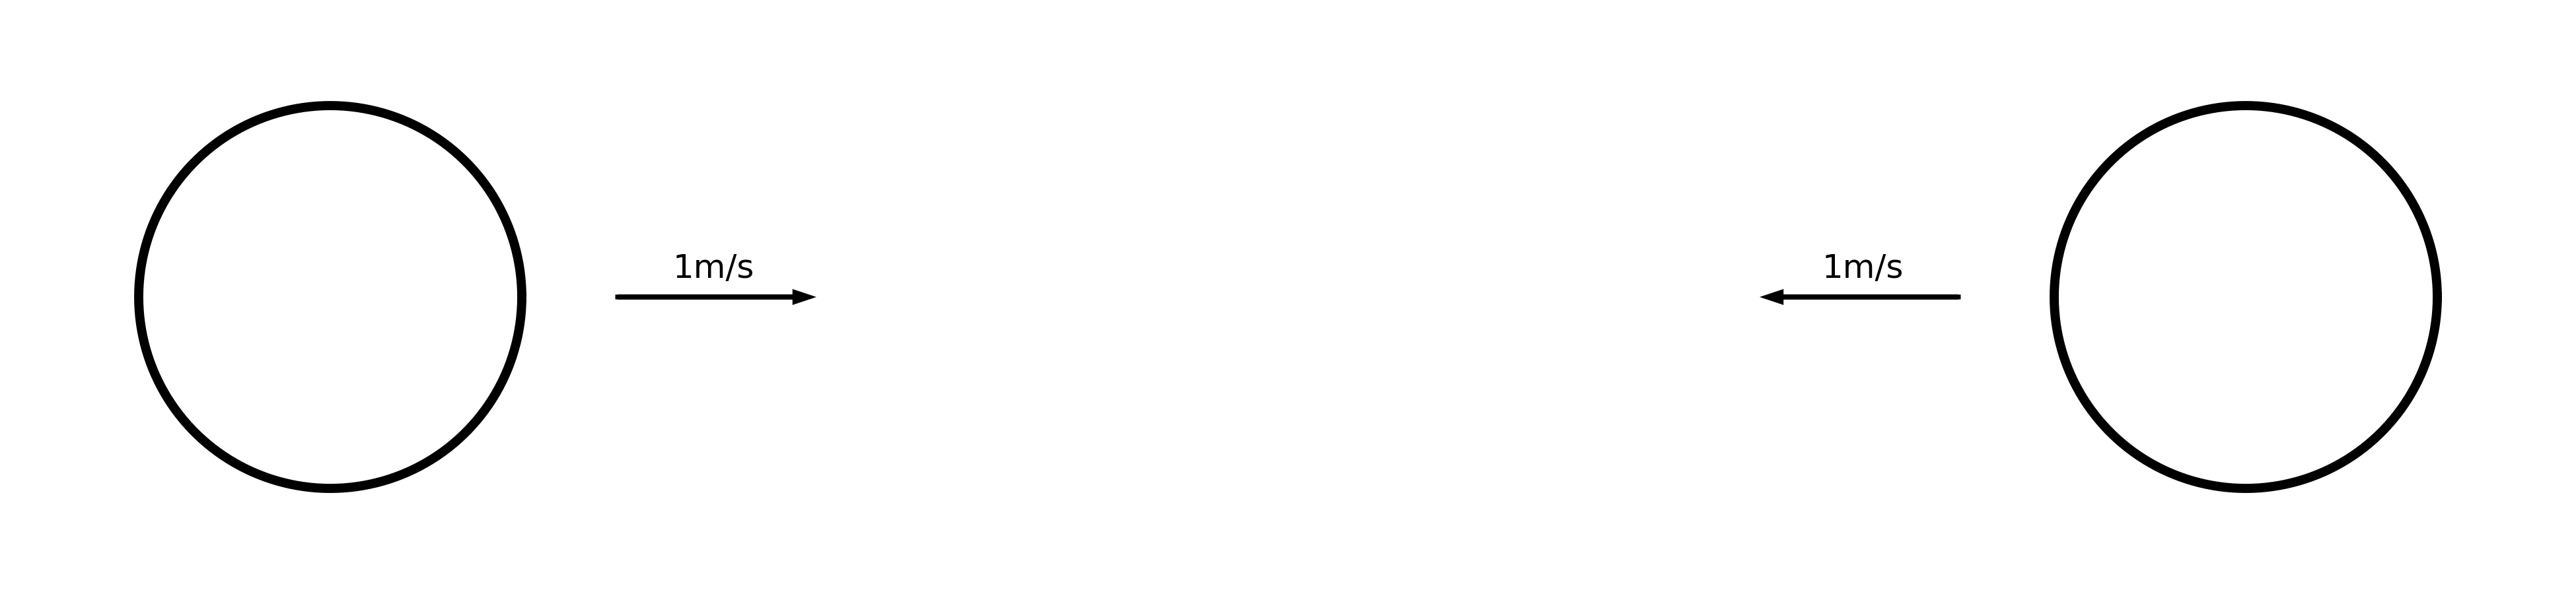
\includegraphics[width=\textwidth]{img1.png}}
\end{center}

Theoretically, the sum of momentum vectors should stay at $(0, 0, 0)$, and the total energy at $\SI{1}{\J}$.
The actual sum of momentum and total energy, as simulated by the engine, will be plotted against time.
The less these values vary, the more accurate the simulation is.

RESULT

\subsubsection{Support test}

SETUP

A box will be placed on a static inclined plane. The coefficient restitution $\epsilon$ is set to be $0$ - this means a perfectly inelastic collision happens between the box and the plane, so the plane should be able to support the ball. Test if the ball could slide down the plane in an accurate manner.

The plane passes through the origin $(0, 0, 0)$ and is sufficiently long to hold the cube. The experiment is mostly within the $x-z$ plane. The cube is 1x1x1, and its center of mass is placed at $(-20\cos \theta + \frac{1}{2}\sin \theta, 0, 20\sin\theta+\frac{1}{2}\cos \theta)$. This means its middle contact point with the plane is always $d=20$m from the origin. Constant gravity $G = \SI{10}{\N}$ will be applied to the cube. At any none $0$ degree angle $(\theta > 0)$, the cube should slide down the plane. The time it takes for the $x$ coordinate of its centre to reach $\frac{1}{2}\sin \theta$ will be measured and checked with the theoretical result. Then the experiment will be repeated for different angles $\theta$ within the range $(0, \frac{\pi}{2})$.

In order to obtain a theoretically perfect result, consider a cube moving frictionless slope. Its acceleration along the slope should be $a=\frac{G}{m}\sin \theta$. If the time it takes when accelerating from a static position is $t$, the distance travelled should be $\frac{1}{2}at^2$. So the theoretical time it takes to reach the origin should be $t_0=\sqrt{\frac{2d}{a}}=\sqrt{\frac{2dm}{G\sin \theta}}=\frac{2}{\sqrt{\sin\theta}}$.

\begin{center}
  \makebox[\textwidth]{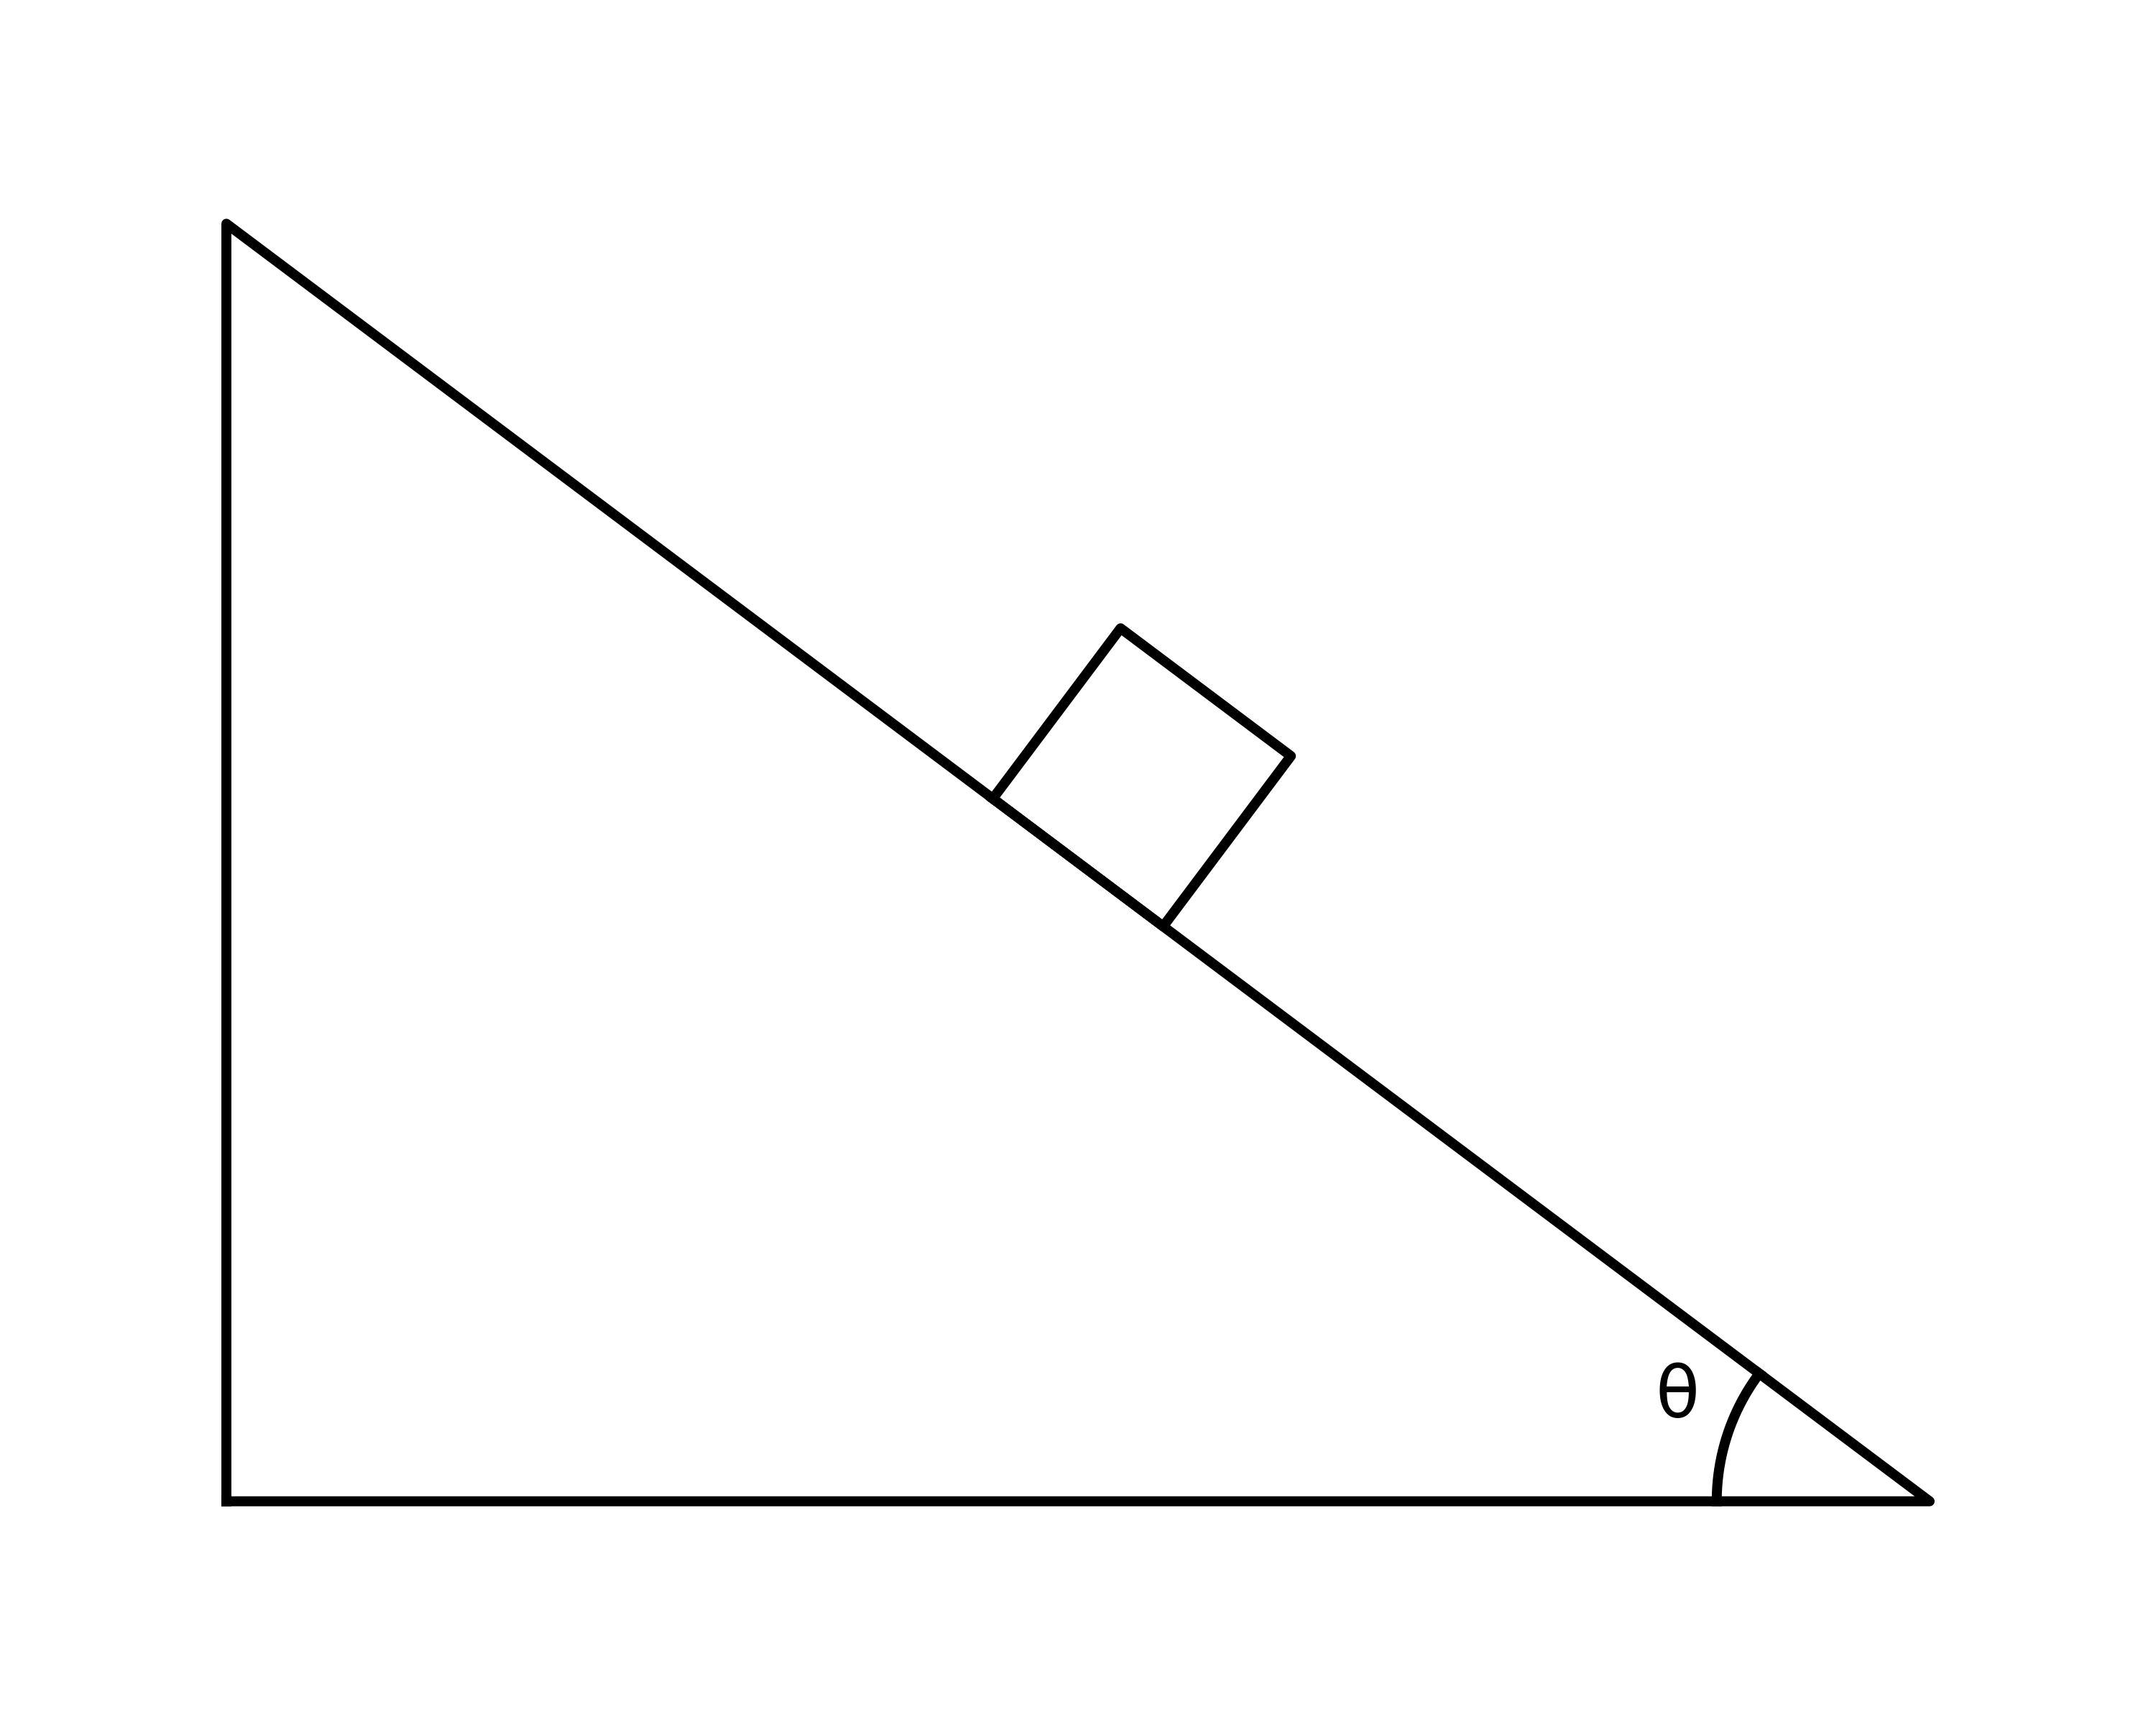
\includegraphics[width=0.5\textwidth]{img2.png}}
\end{center}

RESULT


\subsubsection{Pendulum test}

SETUP

Have a pendulum setup like in the following figure.
A sphere of radius 1m is attached to a fixed point using a bar of radius $\SI{0.001}{\m}$ and length of $\SI{10}{\m}$.
The initial angle between the bar that connects the sphere and an imaginary vertical line through the fixed point is $\theta$.

\begin{center}
    \makebox[\textwidth]{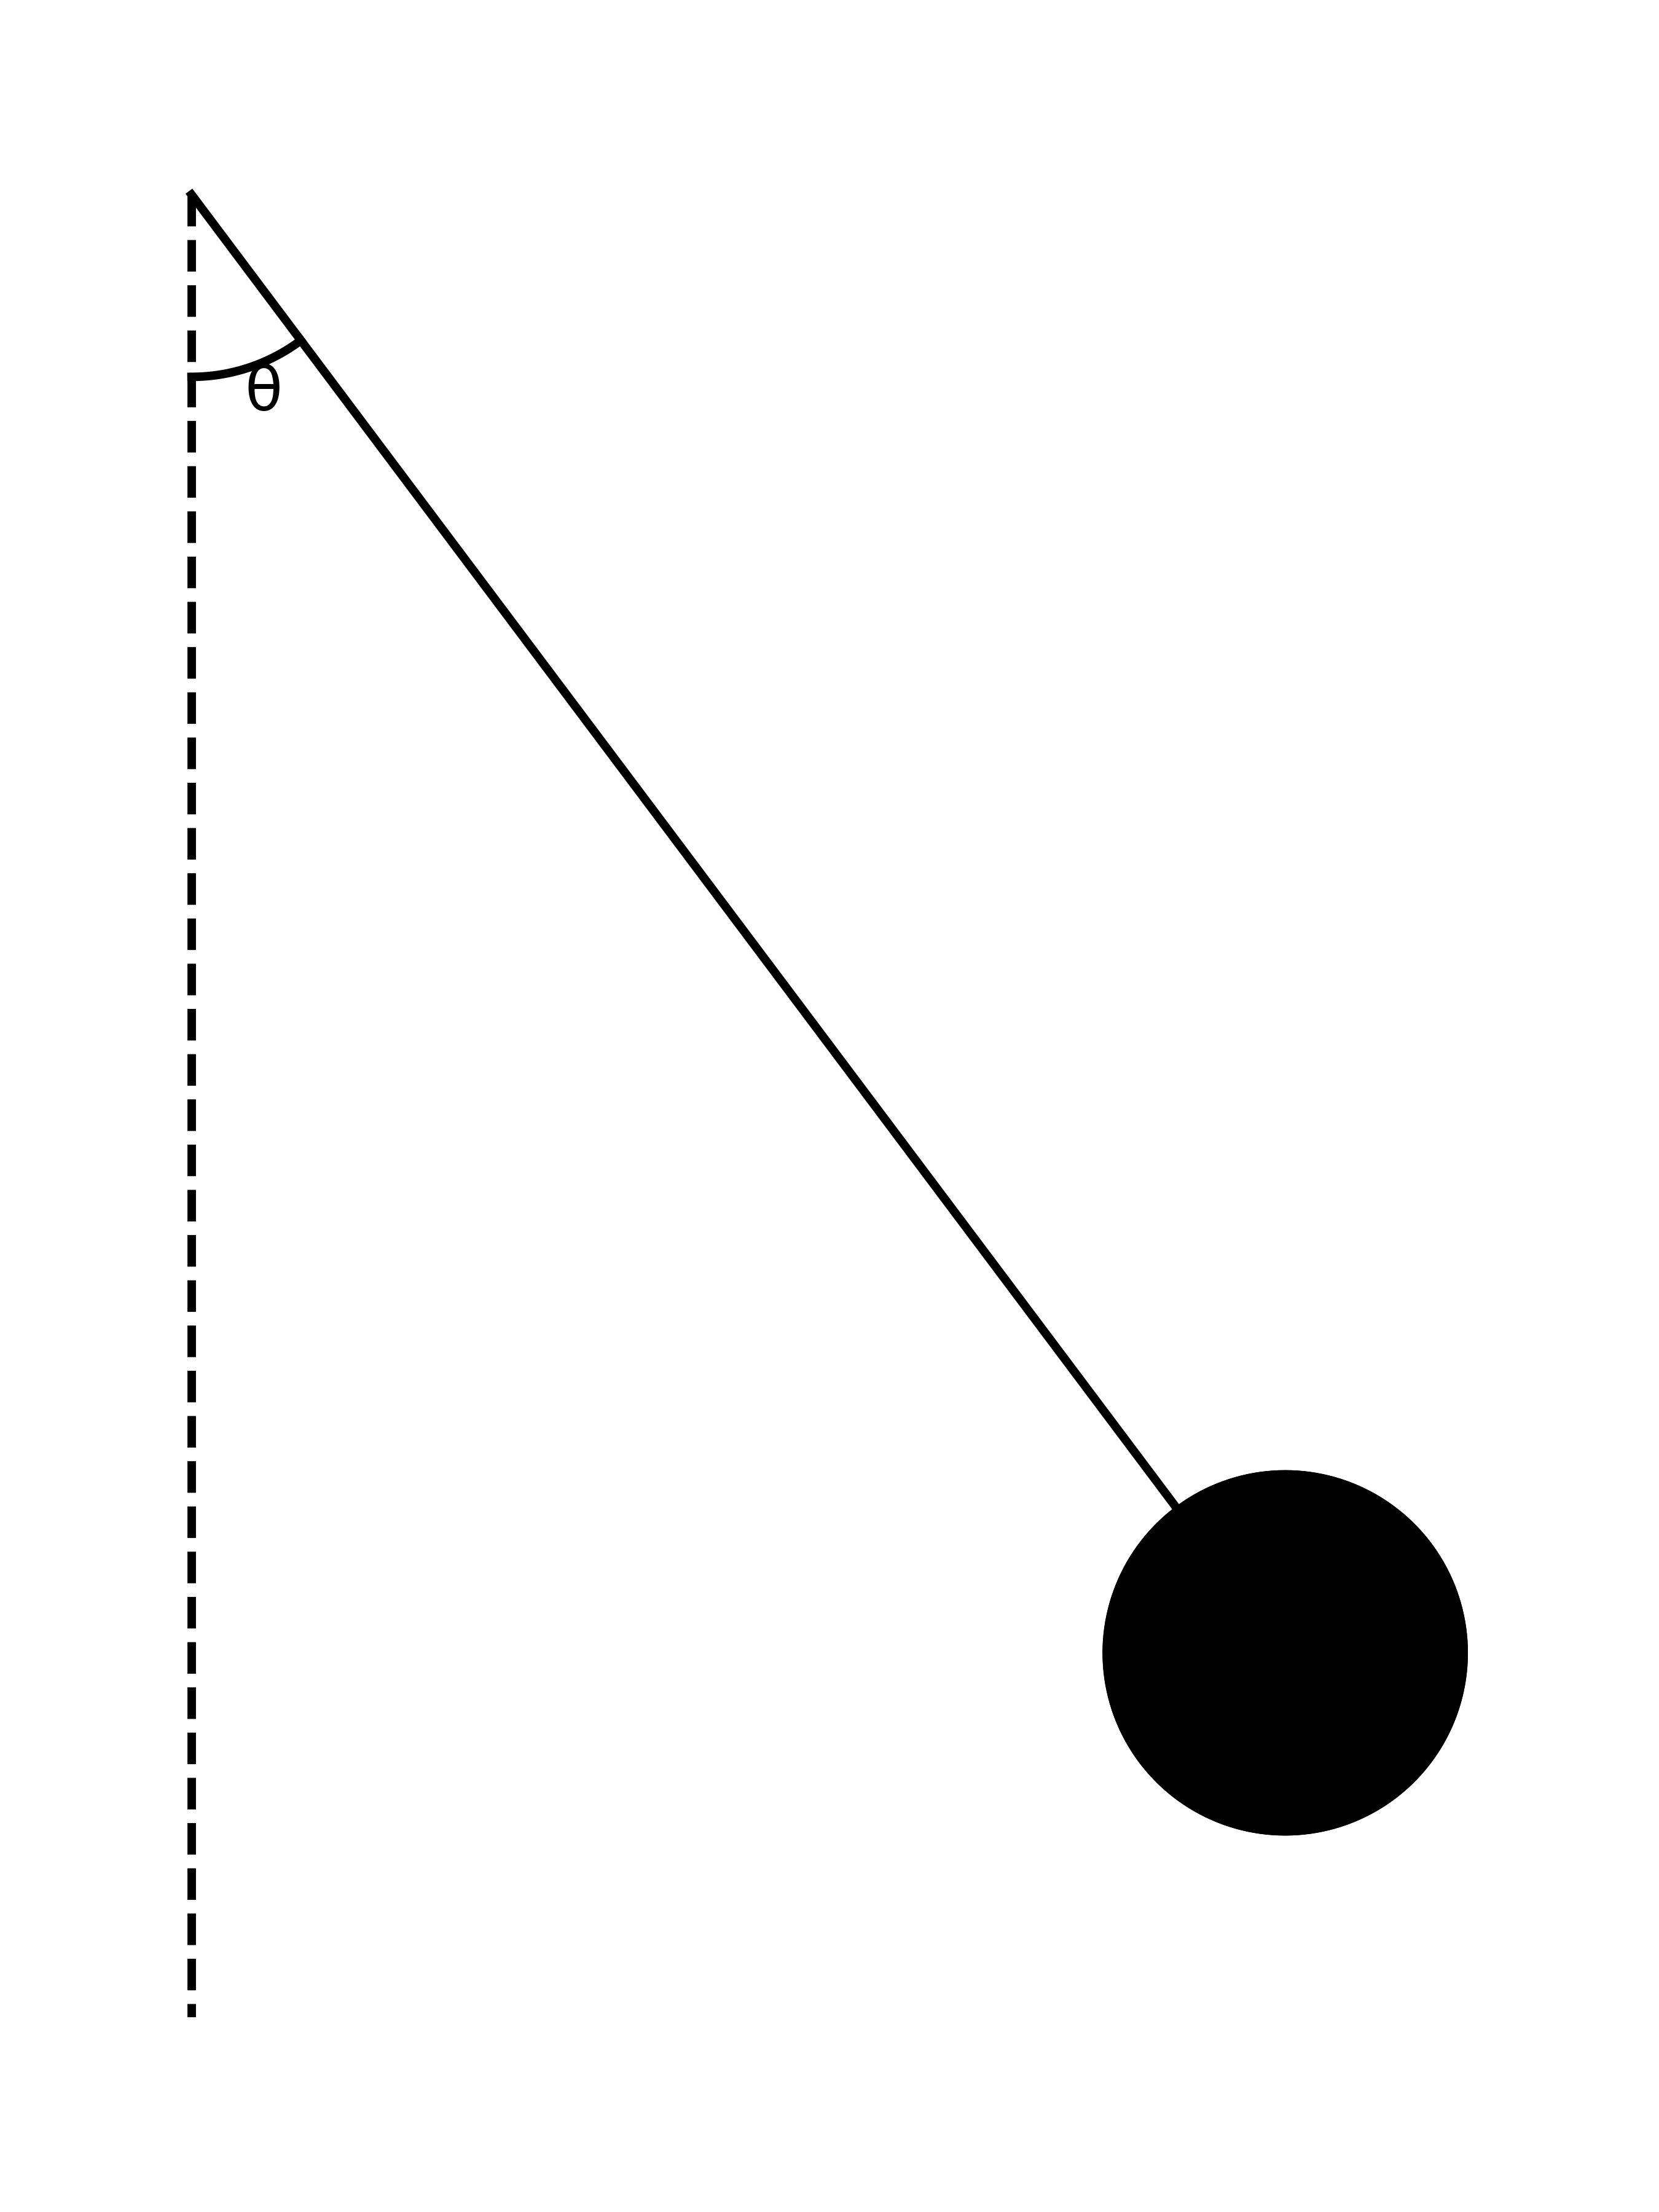
\includegraphics[width=0.3\textwidth]{img3.png}}
  \end{center}

$\theta$ is gradually increased from $5\degree$ to $85\degree$.
For each $\theta$, 
the period of the pendulum is measured by recording the time it takes for the sphere to reach its lowest point $5$ times.

Theoretically, the period of a pendulum is

\begin{equation}
T = 2  \pi \cdot \sqrt{\frac{1}{g}}
\end{equation}

The periods as simulated by the engines will be plotted against the angle $\theta$.

RESULT

\subsubsection{Falling test}

SETUP

The performance of the engine will similarly be measured with a test.

A total number of $n$ cubes, all of size $\SI{1}{\m} \times \SI{1}{\m} \times \SI{1}{\m}$, 
are placed at $(0, 0, \SI{2}{\m}), (0, 0, \SI{4}{\m}), \ldots, (0, 0, (n \times 2)\SI{}{\m})$ above a plane of $z = 0$, 
as shown below.

The masses of each cube is chosen uniformly between $\SI{1}{\kg}$ to $\SI{10}{\kg}$, in order to add complexity.

The average computational time of a time step is measured and plotted against the number of cubes, $n$.
The average computational time is defined as the average of computational time 
it takes for my computer to simulate the scene in the first $n$ seconds.

RESULT

\section{Qualitative analysis}



\noindent\rule{12cm}{0.4pt}

TODO:





\begin{center}
  \makebox[\textwidth]{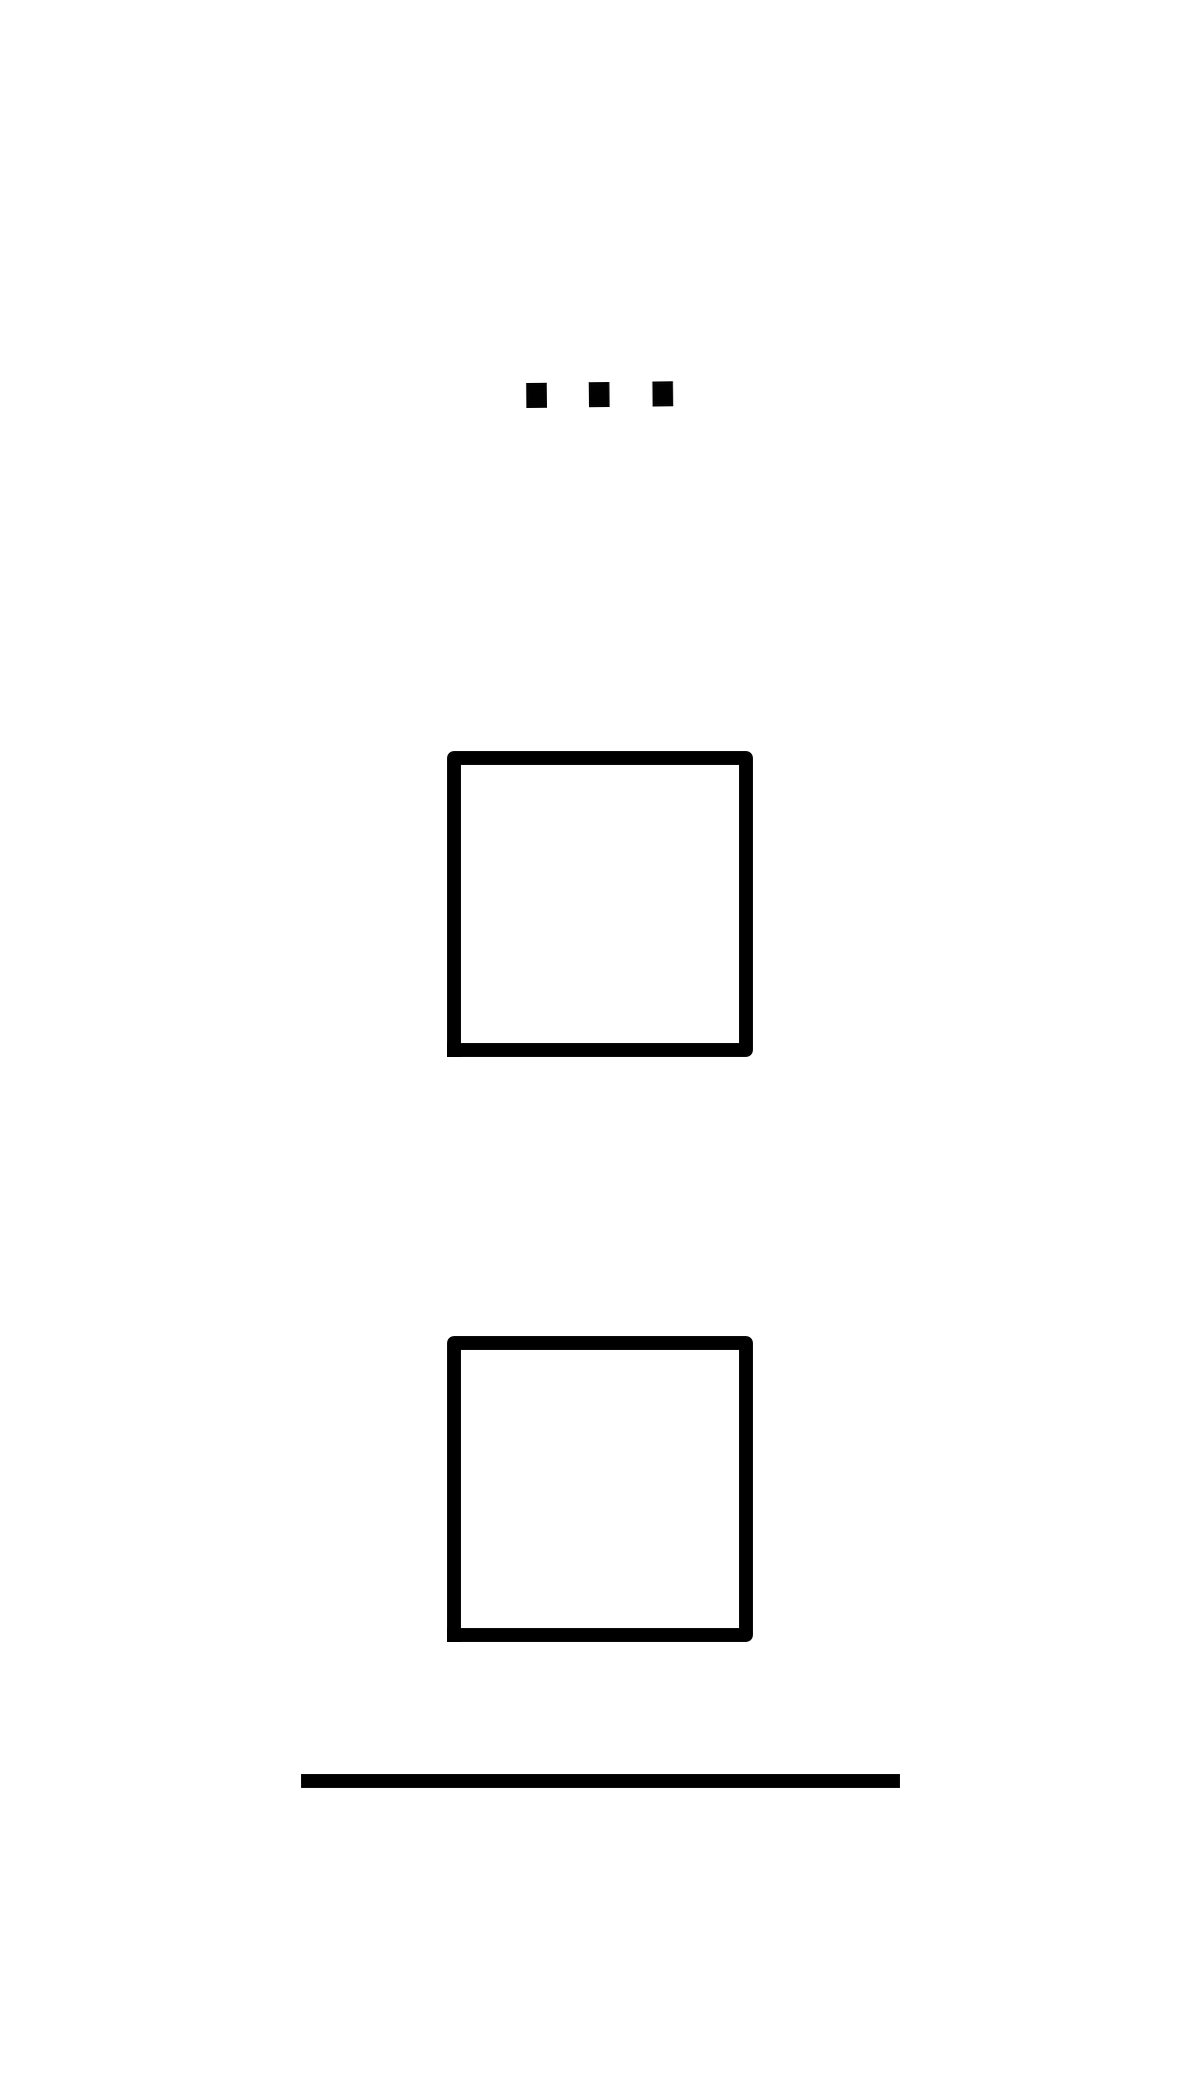
\includegraphics[width=0.3\textwidth]{img4.png}}
\end{center}


\end{document}
